% Options for packages loaded elsewhere
\PassOptionsToPackage{unicode}{hyperref}
\PassOptionsToPackage{hyphens}{url}
%
\documentclass[
  english,
  ,man,floatsintext]{apa6}
\usepackage{lmodern}
\usepackage{amsmath}
\usepackage{ifxetex,ifluatex}
\ifnum 0\ifxetex 1\fi\ifluatex 1\fi=0 % if pdftex
  \usepackage[T1]{fontenc}
  \usepackage[utf8]{inputenc}
  \usepackage{textcomp} % provide euro and other symbols
  \usepackage{amssymb}
\else % if luatex or xetex
  \usepackage{unicode-math}
  \defaultfontfeatures{Scale=MatchLowercase}
  \defaultfontfeatures[\rmfamily]{Ligatures=TeX,Scale=1}
\fi
% Use upquote if available, for straight quotes in verbatim environments
\IfFileExists{upquote.sty}{\usepackage{upquote}}{}
\IfFileExists{microtype.sty}{% use microtype if available
  \usepackage[]{microtype}
  \UseMicrotypeSet[protrusion]{basicmath} % disable protrusion for tt fonts
}{}
\makeatletter
\@ifundefined{KOMAClassName}{% if non-KOMA class
  \IfFileExists{parskip.sty}{%
    \usepackage{parskip}
  }{% else
    \setlength{\parindent}{0pt}
    \setlength{\parskip}{6pt plus 2pt minus 1pt}}
}{% if KOMA class
  \KOMAoptions{parskip=half}}
\makeatother
\usepackage{xcolor}
\IfFileExists{xurl.sty}{\usepackage{xurl}}{} % add URL line breaks if available
\IfFileExists{bookmark.sty}{\usepackage{bookmark}}{\usepackage{hyperref}}
\hypersetup{
  pdftitle={Cognates are advantaged in early bilingual expressive vocabulary development},
  pdfauthor={Lori Mitchell1, Rachel Ka-Ying Tsui1, \& Krista Byers-Heinlein1},
  pdflang={en-EN},
  pdfkeywords={bilingualism, infants, cognates, translation equivalents, phonological similarity, expressive vocabulary development},
  hidelinks,
  pdfcreator={LaTeX via pandoc}}
\urlstyle{same} % disable monospaced font for URLs
\usepackage{graphicx}
\makeatletter
\def\maxwidth{\ifdim\Gin@nat@width>\linewidth\linewidth\else\Gin@nat@width\fi}
\def\maxheight{\ifdim\Gin@nat@height>\textheight\textheight\else\Gin@nat@height\fi}
\makeatother
% Scale images if necessary, so that they will not overflow the page
% margins by default, and it is still possible to overwrite the defaults
% using explicit options in \includegraphics[width, height, ...]{}
\setkeys{Gin}{width=\maxwidth,height=\maxheight,keepaspectratio}
% Set default figure placement to htbp
\makeatletter
\def\fps@figure{htbp}
\makeatother
\setlength{\emergencystretch}{3em} % prevent overfull lines
\providecommand{\tightlist}{%
  \setlength{\itemsep}{0pt}\setlength{\parskip}{0pt}}
\setcounter{secnumdepth}{-\maxdimen} % remove section numbering
% Make \paragraph and \subparagraph free-standing
\ifx\paragraph\undefined\else
  \let\oldparagraph\paragraph
  \renewcommand{\paragraph}[1]{\oldparagraph{#1}\mbox{}}
\fi
\ifx\subparagraph\undefined\else
  \let\oldsubparagraph\subparagraph
  \renewcommand{\subparagraph}[1]{\oldsubparagraph{#1}\mbox{}}
\fi
% Manuscript styling
\usepackage{upgreek}
\captionsetup{font=singlespacing,justification=justified}

% Table formatting
\usepackage{longtable}
\usepackage{lscape}
% \usepackage[counterclockwise]{rotating}   % Landscape page setup for large tables
\usepackage{multirow}		% Table styling
\usepackage{tabularx}		% Control Column width
\usepackage[flushleft]{threeparttable}	% Allows for three part tables with a specified notes section
\usepackage{threeparttablex}            % Lets threeparttable work with longtable

% Create new environments so endfloat can handle them
% \newenvironment{ltable}
%   {\begin{landscape}\centering\begin{threeparttable}}
%   {\end{threeparttable}\end{landscape}}
\newenvironment{lltable}{\begin{landscape}\centering\begin{ThreePartTable}}{\end{ThreePartTable}\end{landscape}}

% Enables adjusting longtable caption width to table width
% Solution found at http://golatex.de/longtable-mit-caption-so-breit-wie-die-tabelle-t15767.html
\makeatletter
\newcommand\LastLTentrywidth{1em}
\newlength\longtablewidth
\setlength{\longtablewidth}{1in}
\newcommand{\getlongtablewidth}{\begingroup \ifcsname LT@\roman{LT@tables}\endcsname \global\longtablewidth=0pt \renewcommand{\LT@entry}[2]{\global\advance\longtablewidth by ##2\relax\gdef\LastLTentrywidth{##2}}\@nameuse{LT@\roman{LT@tables}} \fi \endgroup}

% \setlength{\parindent}{0.5in}
% \setlength{\parskip}{0pt plus 0pt minus 0pt}

% \usepackage{etoolbox}
\makeatletter
\patchcmd{\HyOrg@maketitle}
  {\section{\normalfont\normalsize\abstractname}}
  {\section*{\normalfont\normalsize\abstractname}}
  {}{\typeout{Failed to patch abstract.}}
\patchcmd{\HyOrg@maketitle}
  {\section{\protect\normalfont{\@title}}}
  {\section*{\protect\normalfont{\@title}}}
  {}{\typeout{Failed to patch title.}}
\makeatother
\shorttitle{Cognate advantage in bilingual infants}
\keywords{bilingualism, infants, cognates, translation equivalents, phonological similarity, expressive vocabulary development}
\usepackage{lineno}

\linenumbers
\usepackage{csquotes}
\usepackage{amsmath}
\usepackage[labelformat=empty]{caption}
\usepackage{caption}
\renewcommand{\topfraction}{1}
\renewcommand{\bottomfraction}{1}
\renewcommand{\textfraction}{.1}
\renewcommand{\floatpagefraction}{1}
\setcounter{topnumber}{9}
\setcounter{bottomnumber}{9}
\setcounter{totalnumber}{20}
\setcounter{dbltopnumber}{9}
\ifxetex
  % Load polyglossia as late as possible: uses bidi with RTL langages (e.g. Hebrew, Arabic)
  \usepackage{polyglossia}
  \setmainlanguage[]{english}
\else
  \usepackage[shorthands=off,main=english]{babel}
\fi
\ifluatex
  \usepackage{selnolig}  % disable illegal ligatures
\fi

\title{Cognates are advantaged in early bilingual expressive vocabulary development}
\author{Lori Mitchell\textsuperscript{1}, Rachel Ka-Ying Tsui\textsuperscript{1}, \& Krista Byers-Heinlein\textsuperscript{1}}
\date{}


\affiliation{\vspace{0.5cm}\textsuperscript{1} Concordia University}

\abstract{
Bilingual infants grow up with the unique experience of needing to learn two words for most concepts. These words are called translation equivalents, and translation equivalents that also sound similar (e.g., banana-\emph{banane}) are called cognates. Research has consistently shown that children and adults process cognates more easily than non-cognates. The present study explored if there is such an advantage for cognate production in bilinguals' early vocabulary development. Using longitudinal expressive vocabulary data collected from 47 English--French bilingual infants starting at the ages of 16--20 months up to 27 months (a total of 219 monthly administrations in both English and French), results showed that children produced a greater percentage of cognate words than non-cognate words on the MacArthur-Bates Communicative Development Inventories. Moreover, the magnitude of the cognate advantage increased with age. The findings suggest cognate learning is facilitated in early bilingual vocabulary development. Just as in monolingual infants, these results suggest that phonological overlap supports bilingual language acquisition.
}



\begin{document}
\maketitle

\captionsetup[table]{labelformat=empty}

Infants understand some words during the first year of life, and begin to produce words around their first birthday (Fenson et al., 2007). To do so, infants must represent both the phonological and semantic aspects of a word, and associate the two. Intriguingly, the network of words that children already know appear to shape the words that they will learn: monolingual infants are more likely to learn words that are phonologically (Luce \& Pisoni, 1998; Coady \& Aslin, 2003) and semantically (Coady \& Aslin, 2003) similar to those they already know. Bilingual infants provide a unique perspective into understanding children's developing lexical networks, as they must acquire translation equivalents, which are cross-language synonyms with complete or nearly complete semantic overlap (e.g., ``apple'' in English and \emph{``pomme''} in French; De Houwer et al., 2006; Legacy et al., 2017; Pearson et al., 1995; see White et al.~(2017) for a discussion of convergence in bilinguals' semantic representations). For infants acquiring typologically or historically related languages, some of these translation equivalents will be cognates, which are also phonologically similar (e.g.~``banana'' in English and \emph{``banane''} in French). This current study aimed to understand the impact of cognate status on the acquisition of words in young bilinguals by examining whether bilingual infants produce cognates more readily than non-cognates in early language development.

\hypertarget{translation-equivalents}{%
\subsection{Translation Equivalents}\label{translation-equivalents}}

Translation equivalents are an important part of early language development for bilingual children. While early researchers claimed that bilinguals avoid learning translation equivalents (Volterra \& Taeschner, 1978), more recent work shows that bilingual infants acquire translation equivalents from an early age (Legacy et al., 2017; Pearson et al., 1995). Bilingual infants begin to produce translation equivalents by 16 months, and produce more translation equivalents with age as their vocabulaires grow (Legacy et al., 2017). By the age of 27 months, bilingual toddlers recognize target words more accurately when preceded by its translation equivalent (Floccia et al., 2020).

Some translation equivalents share form and thus phonological overlap between languages, typically due to a shared etymology; these are called cognates. Cognates range in their degree of phonological similarity: For example, English ``banana'' and French \emph{``banane''} are identical except for their last phoneme, while English ``pants'' and French \emph{``pantalon''} differ across multiple phonemes, and even have different number of syllables. Some typologically close languages even have form-identical cognates, such as the word \emph{``si''} which means yes in both Spanish and Catalan.

Cognates appear to have a special status in bilingual language processing. Previous research has reported a cognate facilitation effect where bilinguals are better and quicker at identifying cognates than non-cognates when performing vocabulary tasks (e.g., Costa et al., 2000; Kelley \& Kohnert, 2012; Sheng et al., 2016). This type of advantage for cognates has been reported in bilingual adults (e.g., Costa et al., 2000) as well as in school-aged children (e.g., Kelley \& Kohnert, 2012; Sheng et al., 2016). For example, Kelley and Kohnert (2012) provide evidence for the cognate facilitation effect in Spanish-speaking English-language learners between the ages of eight and 13 years old, where the children identified and named more cognates than non-cognates in receptive and expressive vocabulary tasks. A similar cognate advantage has been found for picture naming and translation tasks for English-Spanish and English-German 4-8 year-old children (Schelletter, 2002; Sheng et al., 2016). Therefore, cognates seem to be advantaged in school-aged bilingual children's language processing and production.

\hypertarget{effects-of-phonological-similarity-on-early-word-learning}{%
\subsection{Effects of Phonological Similarity on Early Word Learning}\label{effects-of-phonological-similarity-on-early-word-learning}}

The advantage for cognates could be attributed to the phonological overlap between words, which may make them easier to learn. Existing literature on monolinguals has reported phonological neighborhood density effects, where monolingual children are more likely to produce words that sound similar to other words in their lexicons (e.g., ``at'' and ``cat,'' ``hat'' and ``cat''), especially at younger ages (e.g., Jones \& Brandt, 2019). For instance, looking at 300 British English-speaking children aged 12 to 25 months, Jones and Brandt (2019) found that the strength of phonological similarity between words was an important predictor for word production (but not comprehension), where young children tended to produce words that follow similar phonological patterns. Similarly, using archival expressive vocabulary data from 1,800 16- to 30-month-old American infants, it was shown that infants produced more nouns with many neighbours than those with few neighbours (Storkel, 2009). It is possible that the high degree of phonological similarity aids word acquisition through sounds already established in the lexicons. For example, Demke et al.~(2002) found that hearing phonological neighbours after learning new words facilitated the production of the new words. Therefore, learning a new word with close phonological neighbours seems to help learners maintain the new word in memory, therefore making similar-sounding words easier to acquire and produce. (e.g., Coady \& Aslin, 2003; Demke et al., 2002; Jones \& Brandt, 2019).

Extending this notion to bilingual infants, some evidence suggests that phonological similarity facilitates vocabulary learning across languages as well. For example, Gampe et al.~(2021) examined parent-reported vocabulary size of 18-36 month-old children learning Swiss German and another language. Children learning languages that were more phonologically similar to Swiss German (e.g., standard German, Dutch, English) produced more words than children learning languages that were more phonologically dissimilar (e.g., Turkish, French). Moreover, children learning more similar languages learned more cognate translation equivalents, while the number of non-cognate translation equivalents was similar across groups. These results are consistent with other studies reporting that language distance affects early bilingual language acquisition (e.g., Blom et al., 2019; Gampe et al., 2021; Havy et al., 2016; Sheng et al., 2016).

However, not all studies have reported a generalized advantage for cognates in vocabulary learning. In a study of younger children, Bosch and Ramon-Casas (2014) used parent report to examine word production in 18-month-olds learning Spanish and Catalan, two strongly related languages that share many form-identical (e.g, ``yes'' is \emph{``si''} in both Spanish and Catalan) and form-similar (e.g., ``hand'' is \emph{``mano''} in Spanish and ``ma'' in Catalan) cognates. Results indicated that 28\% of the words produced by the bilingual infants was composed of form-identical cognates, while less than 2\% of words were form-similar cognates or non-cognate translation equivalents (Bosch \& Ramon-Casas, 2014). One explanation for this finding is that for form-identical cognates, infants only need to learn a single form for a particular concept, which they can then transfer across their languages. Based on these results, bilingual infants may not benefit from cognates' phonological overlap unless that overlap is perfect. Indeed, there is some evidence that Spanish-Catalan infants are somewhat insensitive to phonological distinctions in form-similar cognates (Ramon-Casas et al., 2009; Ramon-Casas \& Bosch, 2010), perhaps even representing them as form-identical. Another interpretation of this result is that the effect of cognates on bilingual vocabulary learning changes across development, which could explain the discrepant results of the 18-month-old sample studied by Bosch \& Ramon-Casas (2014), and the 18-36 month-old sample studied by Gampe et al.~(2021).

\hypertarget{current-study}{%
\subsection{Current study}\label{current-study}}

To better understand the impact of phonological overlap on bilingual infants' vocabulary learning, we examined the production of cognate and non-cognate translation equivalents in French-English bilingual infants. English and French share many form-similar cognates due to historical language contact (Choi, 2019), although few to no form-identical cognates. Despite the presence of cognates, note that they belong to different language families: English is a Germanic language and French is a Romance language.

We collected monthly vocabulary data on English-French bilingual infants' word production starting between the ages of 16--20 months and ending up to 27 months of age using the MacArthur-Bates Web-Communicative Developmental Inventory: Words and Sentences form in American English (Fenson et al., 2007) and Québec French (Trudeau et al., 1999). From these two forms, we limited our analysis to translation equivalent pairs and then classified the pairs according to cognate status (cognate or non-cognate words). We counted children's production of both translation equivalent pairs (e.g., whether produced both ``apple'' and \emph{``pomme''}, or both ``banana'' and \emph{``banane''}, as well as individual words independent of whether children produced its translation equivalent. Since it is not possible to randomly assign our main variable of interest (cognate status), we analyzed both a complete list of cognate and non-cognate words, as well as a carefully selected subset of these cognate and non-cognate words which were matched on age of acquisition and on word category where possible. .

We hypothesized that cognates would be more readily produced by English-French bilinguals than non-cognates. Thus, we predicted that English-French bilingual infants would produce proportionally more translation equivalent words and pairs that were cognates than non-cognates. We likewise anticipated an interaction between cognate status and age, with a stronger effect of cognate status at older ages as the infants' vocabulary size (and the number of translation equivalent words and pairs produced) grew.

\hypertarget{method}{%
\section{Method}\label{method}}

The present research was approved by the Human Research Ethics Committee at Concordia University {[}certification \#10000439{]}. Participation was on a voluntary basis and the families were free to withdraw at any time. The study design was pre-registered at \url{https://osf.io/rh7av}.

\hypertarget{participants}{%
\subsection{Participants}\label{participants}}

The current study comprised data of 50 French--English bilingual infants (26 females) collected from August 2020 to May 2021, as part of a larger ongoing longitudinal study which aims to collect data from 100 bilingual infants. Participating infants were aged between 16 and 20 months at the onset of participation (mean starting age = 17.98 months, SD = 1.15, range = 16.20 -- 20.40), and were aged between 16 to 27 months at their final time of participation (M = 21.96 months, SD = 3.20, range = 16.30 -- 27.14). Participants were recruited from Québec, Canada through government birth lists, social media, and participating families' referrals. Inclusion criteria were the following: full-term pregnancy (i.e., at least 37 weeks of gestation), at normal birth weight (\textgreater{} 2500 grams), and without reported developmental delays or any hearing or vision problems. Bilingual infants were defined as those exposed globally to both English and French at least 10\% to 90\% of the time over the course of their lives, with less than 10\% of exposure to a third language. To capture a wider range of bilingual experience, the bilingual exposure range in this study was broader compared to some bilingual studies (e.g., Morin-Lessard \& Byers-Heinlein, 2019; Sebastián-Gallés \& Bosch, 2009) but similar to the range used in others (e.g., Hoff \& Ribot, 2017; Place \& Hoff, 2011).

In total, parents completed 230 English CDI administrations and 226 French CDI administrations. We retained only cases where both the English and French were completed at the same time point to be able to determine infants' translation equivalent knowledge. These left us with 219 completed administrations from 47 infants. Six infants contributed data at only one time point, and 41 infants contributed data at more than one time point, with participants contributing an average of 4.70 measurements for each language (SD = 2.51, range = 1 -- 10). On average across the 219 administrations, participating infants were exposed to English 48.80\% of the time (SD = 17.30, range = 11 -- 84), to French 50.60\% of the time (SD = 17.70, range = 16 -- 88), and to a third language 0.60\% of the time (SD = 1.50, range = 0 -- 5). Of the 47 bilingual infants, 26 were English-dominant (M = 60.10\% English exposure, SD = 10, range = 49 -- 84), 20 were French-dominant (M = 66.40\% French exposure, SD = 12.70, range = 51 -- 88), and 1 reported equal exposure to both English and French. The average maternal education level was 17.32 years (SD = 2.29, range = 12 -- 23), and 89.40\% of the mothers had completed a university degree or higher.

\hypertarget{measures}{%
\subsection{Measures}\label{measures}}

\hypertarget{web-based-macarthur-bates-communicative-development-inventory-words-and-sentences-web-cdi}{%
\subsubsection{Web-based MacArthur-Bates Communicative Development Inventory: Words and Sentences (Web-CDI)}\label{web-based-macarthur-bates-communicative-development-inventory-words-and-sentences-web-cdi}}

The number of words produced in English and French was obtained monthly via the web-based versions of the MacArthur-Bates Web-Communicative Development Inventories: Words and Sentences form (Web-CDI; \url{https://webcdi.stanford.edu/}), using the American English version (Fenson et al., 2007) and the Québec French adaptation (``Mots et Énoncés''; Trudeau et al., 1999). Our study focused on the vocabulary checklist component of the CDIs, with 680 words in the English version and 664 words in the Québec French version. We asked the caregiver most familiar with the infant's vocabulary in each language to complete the respective version, although following the instructions on the Web-CDI they could seek help from others who often speak the corresponding language with the infant. The English forms were completed by mothers (88\%), fathers (7\%), and both parents (5\%), whereas the French forms were completed by mothers (84\%), fathers (11\%), and both parents (5\%). Thus, most of the time, the same caregiver (usually the mother) filled out the forms. Generally, whichever caregiver completed forms in a particular language did so throughout the study, with the exception of 2 participants (4.30\%) whose English forms were filled out by different caregivers for some administrations, and 3 participants (6.40\%) whose French forms were filled out by different caregivers for some administrations. Infants' demographic information including age and sex was also collected at the start of the Web-CDI.

\hypertarget{language-exposure-questionnaire-leq-using-the-multilingual-approach-to-parent-language-estimates-maple}{%
\subsubsection{Language Exposure Questionnaire (LEQ) using the Multilingual Approach to Parent Language Estimates (MAPLE)}\label{language-exposure-questionnaire-leq-using-the-multilingual-approach-to-parent-language-estimates-maple}}

The infant's language exposure and background was measured with an adaptation of the Language Exposure Questionnaire (LEQ; Bosch \& Sebastián-Gallés, 2001), using the Multilingual Approach to Parent Language Estimates (MAPLE; Byers-Heinlein et al., 2020). During a 15 to 20 minute structured interview, the primary caregiver(s) were asked questions about the infant's language exposure from birth until their current age. This provided a global estimate of the percentage of exposure that the infant had to each of their languages across all contexts.

\hypertarget{procedure}{%
\subsection{Procedure}\label{procedure}}

Data collection for this study began in August 2020 and ended in May 2021, although the start date of participation varied across participants. On the first of each month, links to the English and French Web-CDI forms were sent to the caregivers by email. On the forms, the words that were checked off in previous months were automatically filled in the following months; thus, caregivers only needed to check off the new words that their child produced each month. This was intended to reduce the burden on participants, and increase the response rate. We asked that the Web-CDI forms be completed during the first week of each month. A reminder was sent on the 8th of the month, and an extra week was given for caregivers who had not yet completed the forms. Although caregivers were asked to fill out the forms every month, it was possible for them to skip some months when necessary. Once the forms were completed, caregivers received a brief report about their child's vocabulary knowledge at that time point, including the total number of words that their child produced as well as the breakdown of the categories (such as animals, food, furniture, etc.) for which their child produced words.
At the first data collection time point, caregivers also completed the LEQ questionnaire with a trained research assistant over Zoom. This was repeated every five months to track any potential changes in the infant's language exposure.

\hypertarget{identification-of-translation-equivalents-and-cognates}{%
\subsection{Identification of Translation Equivalents and Cognates}\label{identification-of-translation-equivalents-and-cognates}}

A list of translation equivalents on the English and French forms of the CDI was created by three proficient English-French bilingual adults who carefully examined the English and French versions of the CDIs; a total of 611 translation equivalent pairs were identified (the full list is available at \url{https://osf.io/7fz6c/}; Gonzalez-Barrero et al., 2020). Next, bilingual research assistants identified 138 of the possible 611 translation equivalent pairs as cognates, with the remaining 473 words as non-cognates. Finally, to obtain a more precise measure of the phonological similarity of the identified cognates, bilingual undergraduate students then performed a similarity rating procedure and ranked recordings of the cognates based on how similar recordings of these words sounded. This method was preferred to other methods that focus on orthography (overlap in spelling), since infants acquire language through spoken words as opposed to reading. These steps were carried out in the Concordia Infant Research Laboratory for different projects, prior to the current study.

From the list of 611 translation equivalents, we further excluded any translation equivalent pairs that had complex relationships rather than one-to-one mappings. For example, ``noodle'' forms a translation equivalent pair with either the French word \emph{``nouilles''} or \emph{``pâtes''}. These pairs were removed because we could not know which form (e.g., \emph{``nouilles''} or \emph{``pâtes''}) the infant produced, and we were not able to classify these pairs as either cognates or non-cognates. This left a complete list of 537 translation equivalents (131 cognates and 406 non-cognates).

Note that the cognates and non-cognates in this list could vary systematically on correlated factors including variations in parts of speech and differences in age of acquisition of certain words between languages. Within the full list of translation equivalents, we thus identified a matched subset of cognates and non-cognates.

The matched list was first restricted to nouns as infants show a noun bias in language acquisition (Caselli et al., 1995), and doing so matched the cognates and non-cognates for part of speech. Next, the remaining 272 translation equivalents (cognates = 90, non-cognates = 182) were matched on age of acquisition and word category where possible (e.g., food, furniture, etc.). However, data on age of acquisition was not available for 41 translation equivalents, which were therefore removed, leaving 231 possible items (cognates = 81, non-cognates = 150). Using the optmatch package (Version 0.9.14; Hansen \& Klopfer, 2006) in the R statistical language (R Core Team, 2019), each cognate item was matched to a non-cognate item according to the typical age of acquisition in both English and French obtained from the wordbankr package (Version 0.3.1; Braginsky, 2018) with the closest match possible on word category. There were 52 pairs that matched exactly based on these criteria. For example, the cognate pair ``chair''--\emph{``chaise''} and the non-cognate pair ``bed''--\emph{``lit''} matched because they are typically acquired at age 21 months in English and French and are both in the furniture category (Braginsky, 2018). The remaining 29 pairs were matched on age of acquisition as well, allowing a possible one-month deviation in either English, French or both. For example, the cognate pair ``mittens''--\emph{``mitaine''} and the non-cognate pair ``slipper''--\emph{``pantoufle''} matched since the English words are acquired at 28 and 27 months respectively (one-month deviation), both French words are acquired at 22 months of age (Braginsky, 2018), and both are clothing. Thus, the final items (81 cognates, 81 non-cognates) included in the matched list were as similar as possible in all respects except their cognate status.

\hypertarget{analytical-strategy}{%
\subsection{Analytical Strategy}\label{analytical-strategy}}

Analyses were run on two different dependent variables to examine whether bilingual infants would produce more cognates than non-cognates over their vocabulary development. The first dependent variable was the overall number of words bilingual infants produced and whether they would produce more cognate words than non-cognate words in general. Infants were therefore given a score of 1 for each word they produced. For example, in the translation equivalent pair ``banana''--\emph{``banane''}, the infant received a score of one for producing either ``banana'' or \emph{``banane''}, a score of two if they could produce both ``banana'' and \emph{``banane''}, and a score of zero if neither word in the pair was produced. For the second dependent variable, we looked at the number of translation equivalent pairs bilingual infants produced and whether they would produce more cognate pairs than non-cognate pairs across English and French. Infants were given a score of 1 only if both the English and French words in a translation equivalent pair were produced. For example, if the infant produced both ``banana'' and \emph{``banane''}, they were given a score of one for knowing this translation equivalent pair; if only one word of the pair was produced (only ``banana'' or only \emph{``banane''}) or neither word in the pair was produced, the infant were given a score of 0 for that translation equivalent pair.

For each dependent variable we conducted analyses using (1) the complete list of cognates and non-cognates (537 translation equivalents pairs in total) and then restricted the analysis to (2) a matched list (nouns only and matched on age of acquisition; 162 translation equivalent pairs in total). Based on the two dependent variables and the two sets of words, we therefore ran a total of four models. Linear mixed effects analyses were performed in the R statistical language (Version 4.0.2; R Core Team, 2019) using the lme4 package (Bates et al., 2015). The lmerTest package (Kuznetsova et al., 2017) was used to calculate p-values. Analysis scripts and the data set used in the present study are available at {[}\url{https://osf.io/rh7av/}{]}.

\hypertarget{results}{%
\section{Results}\label{results}}

\hypertarget{descriptive-measures-of-number-of-words-produced}{%
\subsection{Descriptive Measures of Number of Words Produced}\label{descriptive-measures-of-number-of-words-produced}}

Out of the complete list (a possible 537 translation equivalent pairs with 537 × 2 = 1074 words), bilingual infants on average produced a total of 157 words (SD = 158), with a range of 0 -- 709 words, which constituted 14.60\% of the words on the full list. Moreover, bilingual infants produced an average of 39 complete translation equivalent pairs where both the English and French words were produced (SD = 50.61, range = 0 -- 243), which constituted 7.30\% of the translation equivalent pairs on the full list.

Restricting to the matched list which contained 162 translation equivalent pairs with 162 × 2 = 324 words, bilingual infants produced an average of 51 words (SD = 59.71, range = 0 -- 248), which constituted 15.70\% of the words on the matched list. On average, bilingual infants produced a total of 12 complete translation equivalent pairs (SD = 20.77, range = 0 -- 92), which constituted 7.60\% of translation equivalent pairs on the matched list.

\hypertarget{dependent-variable-1-cognate-words-versus-non-cognate-words}{%
\subsection{Dependent Variable 1: Cognate Words Versus Non-Cognate Words}\label{dependent-variable-1-cognate-words-versus-non-cognate-words}}

In this analysis, the dependent variable was the total percentage of words infants produced on the relevant list. Percentage was used as opposed to raw number of words to provide a more comparable description of production of cognates versus non-cognates, since the number of cognate words and non-cognates words differed especially in the complete list. Our predictor variables were age (in days) and cognate status. Age was continuous and was centered at the mean age of 547.6 days (approximately 18 months) for ease of interpretation. Cognate status was categorical with two levels (cognates versus non-cognates) with non-cognates as the reference level. We ran separate models for the complete and matched lists. The initial model specification included a random slope of age and cognate status by participants, which was pruned to a random intercept to achieve model convergence. The final model was:

percentage\_word \textasciitilde{} age * cognate\_status + (1\textbar participant)

\hypertarget{complete-list}{%
\subsubsection{Complete List}\label{complete-list}}

Out of the complete list which contained 262 cognate words (i.e., adding the 131 English cognate words and 131 French cognate words) and 812 non-cognate words (i.e., adding the 406 English non-cognate words and 406 French non-cognate words), bilingual infants produced an average of 54 cognate words (SD = 45.56, range = 0 -- 204) and 103 non-cognate words (SD = 113.09, range = 0 -- 505). The percentage of cognate words produced was 20.60\% (SD = 17.39, range = 0 -- 77.86), whereas the percentage of non-cognate words produced was 12.68\% (SD = 13.93, range = 0 -- 62.19). Table 1 shows the coefficient estimates for the model and Figure 1 Panel A visualizes the model. The main effect of cognate status was also significant, suggesting that bilingual infants produced 8\% more cognate words than non-cognate words at the mean age of 547.6 days (approximately 18 months). The significant effect of age suggested that for every day of increased age, older infants produced 0.10\% more non-cognate words (the reference level) than younger infants. The significant interaction between age and cognate status further suggested that the pattern of infants producing more cognate words strengthened as they aged, indicating that for every additional day infants produced 0.03\% more cognate words than non-cognate words. As an example, at the youngest age in our sample (\textasciitilde16 months or 493 days), the model predicts little to no difference in cognate vs.~non-cognate production, versus at the oldest age in our sample (\textasciitilde28 months or 826 days), the model predicts that infants will produce 15.67\% more cognates than non-cognates.

\hypertarget{matched-list}{%
\subsubsection{Matched List}\label{matched-list}}

Out of the 162 cognate (i.e., adding the 81 English cognate words and 81 French cognate words) and 162 non-cognate words (i.e., adding the 81 English non-cognate words and 81 French non-cognate words) on the matched list, bilingual infants produced an average of 27 cognate words (SD = 31.52, range = 0 -- 135) and 23 non-cognate words (SD = 28.40, range = 0 -- 113). The overall mean percentage of cognate words produced was 16.90\% of words (SD = 19.46, range = 0 -- 83.33), whereas the percentage of non-cognate words produced was 14.50\% (SD = 17.53, range = 0 -- 69.75). Table 1 also shows the coefficient estimates for the matched list model and Figure 1 Panel B visualizes the model. Similar to the patterns reported in the complete list model, there were significant effects of age and cognate status. The effect of cognate status suggested that in general bilingual infants produced 2\% more cognate words than non-cognate words at the mean age of our sample (547.6 days). The age effect suggested that older infants produced 0.10\% more non-cognate words (the reference level) than younger infants. The interaction between cognate and age was also significant: for every additional day infants produced 0.02\% more cognate words than non-cognate words on the matched list. Therefore, overall the direction of effects was similar to the previous analysis (i.e., more cognate words than non-cognate words).

~

\begin{figure}

{\centering 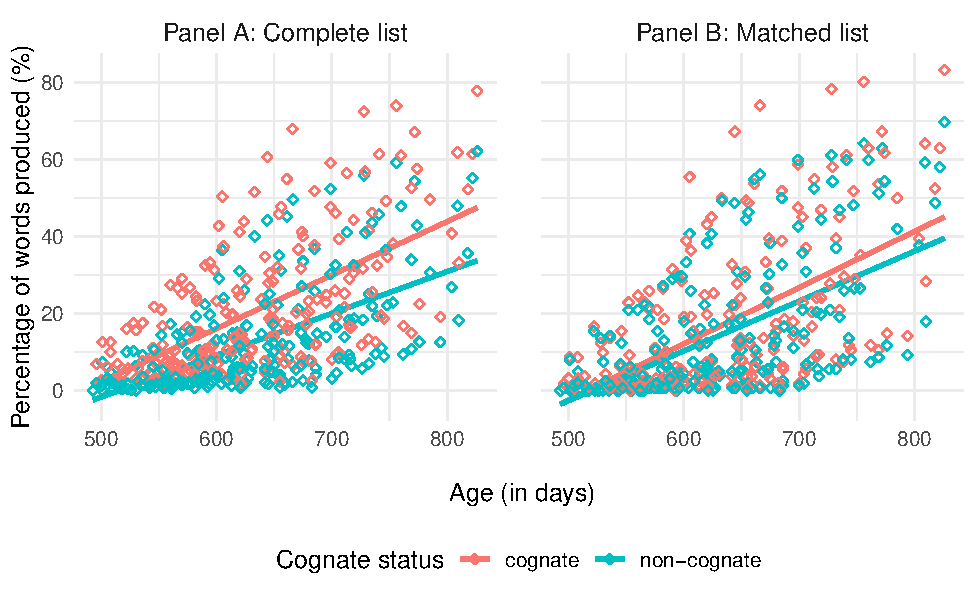
\includegraphics[width=1.2\linewidth]{CogVocab_paper_files/figure-latex/Fig1-1} 

}

\caption{Percentage of words produced by age and cognate status, with Panel A representing the complete list and Panel B representing the matched list.}\label{fig:Fig1}
\end{figure}

\begin{lltable}

\begin{longtable}{lcccccccccl}\noalign{\getlongtablewidth\global\LTcapwidth=\longtablewidth}
\caption{\label{tab:Table 1}Table 1. Coefficient estimates from the linear mixed-effects models predicting percentage of words produced.}\\
\toprule
 & \multicolumn{5}{c}{Complete list} & \multicolumn{5}{c}{Matched list} \\
\cmidrule(r){2-6} \cmidrule(r){7-11}
 & Estimate & $df$ & $SE$ & $t$ & $p$ & Estimate & $df$ & $SE$ & $t$ & $p$\\
\midrule
\endfirsthead
\caption*{\normalfont{Table \ref{tab:Table 1} continued}}\\
\toprule
 & \multicolumn{5}{c}{Complete list} & \multicolumn{5}{c}{Matched list} \\
\cmidrule(r){2-6} \cmidrule(r){7-11}
 & Estimate & $df$ & $SE$ & $t$ & $p$ & Estimate & $df$ & $SE$ & $t$ & $p$\\
\midrule
\endhead
Intercept & 13.00 & 1.57 & 49.35 & 8.26 & <.001 & 14.80 & 1.89 & 49.90 & 7.83 & <.001\\
cognate\_status & 7.92 & 0.45 & 389.13 & 17.50 & <.001 & 2.39 & 0.58 & 389.35 & 4.11 & <.001\\
age\_days & 0.11 & 0.00 & 398.57 & 22.40 & <.001 & 0.13 & 0.01 & 400.06 & 20.60 & <.001\\
cognate\_status * age\_days & 0.03 & 0.01 & 389.13 & 5.21 & <.001 & 0.02 & 0.01 & 389.35 & 2.18 & <.05\\
\bottomrule
\end{longtable}

\end{lltable}

\hypertarget{dependent-variable-2-cognate-pairs-versus-non-cognate-pairs}{%
\subsection{Dependent Variable 2: Cognate Pairs Versus Non-Cognate Pairs}\label{dependent-variable-2-cognate-pairs-versus-non-cognate-pairs}}

In this analysis, percentage of translation equivalent pairs produced was entered as the dependent variable. Age and cognate status were entered as our predictor variables, with non-cognates set as the reference level. Again, we ran separate models for the complete and matched lists. The initial model specification, which included a random effect of age and cognate status by participants, had to be reduced for model convergence; therefore, the final model was:

percentage\_pair \textasciitilde{} age * cognate\_status + (1\textbar participant)

\hypertarget{complete-list-1}{%
\subsubsection{Complete List}\label{complete-list-1}}

Out of the complete list which contained 537 translation equivalent pairs (131 cognates and 406 non-cognates), infants produced an average of 17 cognate pairs (SD = 18.10, range = 0 -- 82) and 22 non-cognate pairs (SD = 32.93, range = 0 -- 167). The percentage of cognate pairs produced was 13\% (SD = 13.82, range = 0 -- 62.60) whereas the percentage of non-cognate pairs produced was 5.50\% (SD = 8.11, range = 0 -- 41.13). Table 2 shows the coefficient estimates for the model and Figure 2 Panel A visualizes the model. The significant effect of age suggested that bilingual infants produced 0.06\% more non-cognate pairs (the reference level) with every increase in day of age. There was also a significant effect of cognate status, suggesting that on average infants produced 8\% more translation equivalent pairs that are cognates than those that are non-cognates at the reference age level of 547.6 days. Likewise, the significant interaction between age and cognate status indicated that the pattern of producing more cognate pairs strengthened as bilingual infants aged. Therefore, bilingual infants produced an even greater percentage of cognate pairs than non-cognate pairs with age.

\hypertarget{matched-list-1}{%
\subsubsection{Matched List}\label{matched-list-1}}

Out of the 162 translation equivalent pairs, bilingual infants produced an average of 7 cognate pairs (SD = 12.21, range = 0 -- 58) and 5 non-cognate pairs (SD = 8.83, range = 0 -- 42). The percentage of cognate pairs produced was 9.20\% (SD = 15.07, range = 0 -- 71.60) and the percentage of non-cognate pairs produced was 5.90\% (SD = 10.91, range = 0 -- 51.85). The coefficient estimates for the matched list model is shown in Table 2, and Figure 2 Panel B visualizes the model. Similar to the results for the complete list, the main effects of age and cognate status were significant, as well as the interaction between age and cognate status. The age effect suggested that bilingual infants produced 0.07\% more non-cognate translation equivalent pairs with every day of age. The significant effect of cognate status suggested that overall bilingual infants produced 3\% more cognate translation equivalent pairs than non-cognate pairs at the mean age of our sample (547.6 days). This pattern strengthened with age as suggested by the significant interaction between age and cognate status, such that bilingual infants produced a greater percentage of cognate pairs than non-cognate pairs as they aged.

~

\begin{figure}

{\centering 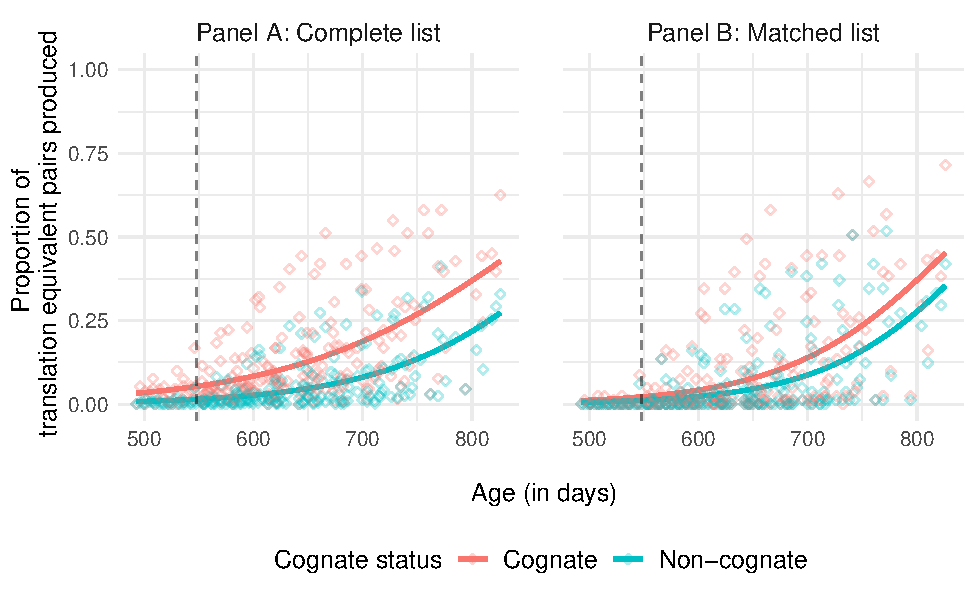
\includegraphics[width=1.2\linewidth]{CogVocab_paper_files/figure-latex/Fig2-1} 

}

\caption{Percentage of translation equivalent pairs produced by age and cognate status, with Panel A representing the complete list and Panel B representing the matched list.}\label{fig:Fig2}
\end{figure}

\begin{lltable}

\begin{longtable}{lcccccccccl}\noalign{\getlongtablewidth\global\LTcapwidth=\longtablewidth}
\caption{\label{tab:Table 2}Table 2. Coefficient estimates from the linear mixed-effects models predicting percentage of translation equivalent pairs produced.}\\
\toprule
 & \multicolumn{5}{c}{Complete list} & \multicolumn{5}{c}{Matched list} \\
\cmidrule(r){2-6} \cmidrule(r){7-11}
 & Estimate & $df$ & $SE$ & $t$ & $p$ & Estimate & $df$ & $SE$ & $t$ & $p$\\
\midrule
\endfirsthead
\caption*{\normalfont{Table \ref{tab:Table 2} continued}}\\
\toprule
 & \multicolumn{5}{c}{Complete list} & \multicolumn{5}{c}{Matched list} \\
\cmidrule(r){2-6} \cmidrule(r){7-11}
 & Estimate & $df$ & $SE$ & $t$ & $p$ & Estimate & $df$ & $SE$ & $t$ & $p$\\
\midrule
\endhead
Intercept & 5.74 & 1.08 & 53.28 & 5.30 & <.001 & 6.17 & 1.27 & 55.06 & 4.86 & <.001\\
cognate\_status & 7.53 & 0.46 & 390.43 & 16.40 & <.001 & 3.29 & 0.59 & 391.12 & 5.53 & <.001\\
age\_days & 0.06 & 0.00 & 408.89 & 12.20 & <.001 & 0.07 & 0.01 & 412.44 & 11.90 & <.001\\
cognate\_status * age\_days & 0.04 & 0.01 & 390.43 & 7.58 & <.001 & 0.03 & 0.01 & 391.12 & 3.93 & <.001\\
\bottomrule
\end{longtable}

\end{lltable}

\hypertarget{summary-of-analyses}{%
\subsection{Summary of Analyses}\label{summary-of-analyses}}

Taken together, our two sets of analyses revealed that overall bilingual infants produced more cognates than non-cognates. This pattern is modulated by age, where bilingual infants produced increasingly more cognates than non-cognates over time. This result was consistent not only across the two sets of analyses, but also across the complete and the matched list.

\hypertarget{discussion}{%
\section{Discussion}\label{discussion}}

This current study evaluated whether phonological similarity facilitates vocabulary learning in bilinguals, by examining whether cognates are advantaged in bilingual infants' early vocabulary production. Using monthly expressive vocabulary data, our longitudinal dataset revealed an advantage for cognates in infancy and its magnitude was modulated by age. Infants produced proportionally more cognates (e.g., English ``banana''--French \emph{``banane''}) than non-cognates (e.g., English ``apple''--French \emph{``pomme''}) over time, although note that in raw terms children still produced more non-cognates than cognates as fewer translation equivalents are cognates than non-cognates for this language pair (i.e., translation equivalents such as ``banana''--\emph{``banane''} are less common than ``apple''--\emph{``pomme''}) . Crucially, the production advantage found for cognates is unlikely to be due to confounding factors, since the same pattern of results was consistently found independent of whether one or both words in a translation equivalent pair are learned, as well as in a carefully matched list of translation equivalents that were matched for part of speech, typical age of acquisition, and word category when possible.

The advantage for cognates observed in bilingual children is likely to be due to an interconnected network between bilinguals' two languages. Previous studies have documented that words from bilinguals' two languages are in fact linked and are processed in parallel. For example, cross-language priming studies on young bilingual children demonstrated that words in both languages were simultaneously activated when bilingual children were using related words in either language and this coactivation begins to emerge from 18 months (e.g., De Anda \& Friend, 2020; Jardak \& Byers-Heinlein, 2018; Singh, 2014). Moreover, phonology plays a role in this interconnected network, as similar-sounding words are coactivated upon hearing a phonologically-related word in one of the two languages (Von Holzen \& Mani, 2012). In other words, words that are semantically- or phonologically-related are linked across bilinguals' two languages. It has been suggested that children more easily learn words that share associative cues and words acquired in one language facilitate the acquisition in bilingual children's other languages (Bilson et al., 2015). Cognates are possibly easier to learn than non-cognates because cognates share more associative cues. While both cognates and non-cognates share semantic overlap across languages, cognates share an additional phonological overlap. In other words, the phonological similarity in cognates facilitates vocabulary acquisition across languages.

Together with previous findings, our results begin to paint a developmental picture of the effects of cognate status on early vocabulary productions. Our results, as well as those of Bosch \& Ramon-Casas (2014) indicate that vocabulary facilitation for form-similar cognates is either difficult to detect or absent at 18 months. Form-identical cognates may be already advantaged by 18 months (Bosch \& Ramon-Casas, 2014), although this could not be examined in our study due to the paucity of form-identical cognates in French and English. From 18--27 months, our data indicate that bilingual children acquire form-similar cognates at a faster rate than non-cognates.

Our findings can, at least in part, explain why bilingual children learning more similar languages show accelerated vocabulary development relative to bilinguals acquiring less similar languages (Blom et al., 2020; Gampe et al., 2021; Sheng et al., 2016). For those who are learning close language pairs like Spanish and Catalan, their two languages share many words that are very similar-sounding to one another --- sometimes share the identical forms (e.g, \emph{``si''} meaning `yes' in both languages). Form-identical cognates are likely to be more salient and frequent in the input and thus easier to acquire than form-similar cognates or non-cognates as only one form needs to be acquired for both languages (Bosch \& Ramon-Casas, 2014). On the other hand, for those who are learning languages that share a lesser degree of phonological similarity like English and French, there would be fewer cognates available, and potentially very few form-identical cognates. Therefore, it is possible that when languages are very similar and share many form-identical cognates, these types of cognates will be acquired preferentially by the infants, but when languages are somewhat less similar and share mostly form-similar cognates, these will be acquired preferentially instead. Future studies could include additional language pairs which are less similar than Spanish and Catalan but more similar than English and French, such as Spanish and Italian (Schepens et al., 2013), to directly compare the acquisition of form-identical cognates, form-similar cognates, and non-cognates.

Despite the difference in the nature, the robust cognate advantage across different bilingual infant populations points to the possibility that the origin of the cognate facilitation effect observed in childhood and in adulthood emerges from infancy. Previous studies which examined the cognate facilitation effect in bilingual adults and school-aged children have reported that bilinguals are better at processing cognates; for example, they can identify and/or name cognates more easily and quickly in a vocabulary task (Costa et al., 2000; Kelley \& Kohnert, 2012; Sheng et al., 2016). Thus, the cognate facilitation effect appears to be robust in vocabulary production across the lifespan, with the advantage for cognates in production emerging early on, as our study results suggested.

An important avenue for future research would be to examine whether the same cognate advantage would apply to receptive vocabulary, and indeed some evidence points in this direction. Young bilingual infants show less perceptual sensitivity to cross-language phonological distinctions in cognates due to their phonological similarity (Ramon-Casas et al., 2009; Ramon-Casas \& Bosch, 2010), suggesting that cognates may hold a different status in early bilinguals' receptive lexicons compared to non-cognates. There is an overall mixed evidence for whether the effect of cognate status is absent in comprehension (Schott \& Byers-Heinlein, 2019) or is present in both comprehension and production (Kelley and Kohnert, 2012). However, it is possible that the cognate advantage is modulated by the level of difficulty of the vocabulary item for both comprehension and production. It has been found that although the cognate advantage was found in easier items, the effect was even greater in vocabulary items that were considered to be medium or hard (Kelley \& Kohnert, 2012). This may suggest that infants would have a cognate advantage in any sort of task, especially for less-familiar words where they may use the cognate word they have already acquired for help (Kelley \& Kohnert, 2012), which is the case when infants are acquiring new words and learning to pronounce them. Therefore, we could expect a cognate advantage in both comprehension and production, serving different purposes: in comprehension, a cognate advantage would help activate the representations for the words in both languages, whereas in production, cognates may facilitate the acquisition of the word in the individuals' other language in terms of pronunciation, as was seen in our study. Future research could explore the difference between comprehension and production in bilingual infants' language acquisition while simultaneously looking at the cognate advantage.

\hypertarget{conclusion}{%
\section{Conclusion}\label{conclusion}}

The present study demonstrated thatEnglish-French bilingual infants' show an advantage for cognates in vocabulary production, with proportionally more cognates being produced than non-cognates, a pattern which magnified as the infants grew older and learned more vocabulary. This finding can, at least in part, explain why children learning typologically similar languages show faster vocabulary growth than those learning more distant languages (Blom et al., 2020; Gampe et al., 2021; Sheng et al., 2016). Altogether, our study provides a greater understanding of the effect of similar-sounding words on infants' language acquisition over time. Future studies with data from other populations of bilinguals will be important to more fully understand the effect of the cognate advantage in early bilingual vocabulary development.


\end{document}
